\documentclass[11pt, a4paper]{article}

% ----- Packages -----
\usepackage[utf8]{inputenc}
\usepackage[T1]{fontenc}
\usepackage{geometry}
\geometry{a4paper, margin=1in}
\usepackage{graphicx}
\usepackage{amsmath, amssymb, amsfonts}
\usepackage{hyperref}
\usepackage{float}
\usepackage{subcaption}
\usepackage{fancyhdr}
\usepackage{xcolor}
\usepackage{microtype}
\usepackage{booktabs}
\usepackage{tcolorbox}
\usepackage{titlesec}

% ----- Styling -----
\definecolor{primary}{RGB}{0, 82, 155} % A nice professional blue
\hypersetup{
    colorlinks=true,
    linkcolor=primary,
    filecolor=magenta,      
    urlcolor=primary,
}

\titleformat{\section}{\large\bfseries\color{primary}}{\thesection}{1em}{}
\titleformat{\subsection}{\normalsize\bfseries}{\thesubsection}{1em}{}

\pagestyle{fancy}
\fancyhf{}
\lhead{\textit{EE200: Course Project}}
\rhead{\textit{Question 3 Report}}
\cfoot{\thepage}

% ----- Document -----
\begin{document}

\begin{titlepage}
    \centering
    \vspace*{2cm}
    
    \Huge
    \textbf{\textcolor{primary}{Sonic Signatures \& Signals to Softwares}}
    
    \vspace{0.5cm}
    \LARGE
    EE200 Course Project: Question 3
    
    \vspace{1.5cm}
    
    \Large
    \textbf{Prepared by:} \\
    Student Name / ID
    
    \vfill
    
    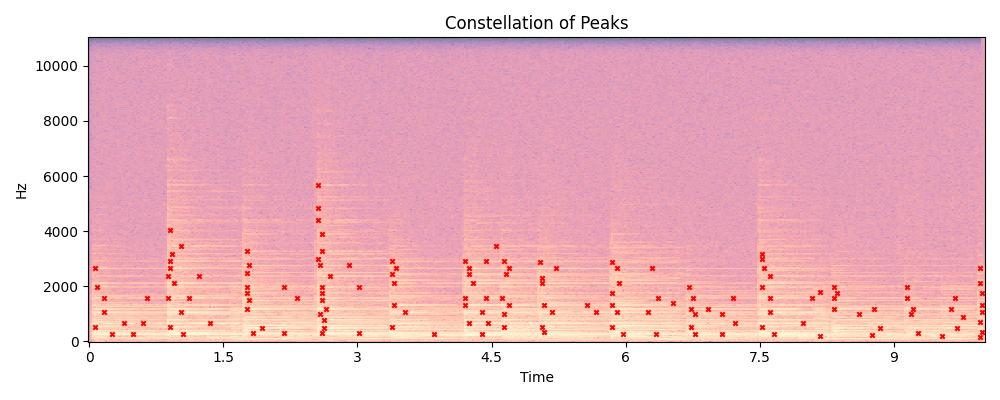
\includegraphics[width=0.4\textwidth]{plots/constellation.png} % Cover image
    
    \vfill
    
    \Large
    \today
    
\end{titlepage}

\newpage
\tableofcontents
\newpage

\begin{abstract}
\noindent This report details the design, implementation, and evaluation of an acoustic fingerprinting and recognition system (akin to Shazam), developed for the EE200 course project. The system processes raw audio signals using the Short-Time Fourier Transform (STFT) to compute spectrograms, extracts a sparse constellation of local maxima, and computes robust time-frequency hashes. Furthermore, an interactive web application was deployed using the Streamlit framework to provide a user-friendly interface for both single-clip and batch recognition tasks. Extensive robustness testing demonstrates the system's resilience to additive white Gaussian noise and highlights an algorithmic enhancement utilizing frequency ratios to achieve true pitch-shift invariance.
\end{abstract}

\section{Methodology: Acoustic Fingerprinting}

\subsection{The Limitation of the Global DFT}
To identify a song, one might initially consider taking the global Discrete Fourier Transform (DFT) of the entire audio signal to extract its frequency content. The magnitude spectrum of the DFT reveals the aggregate frequencies present across the entire track. 

\begin{figure}[H]
    \centering
    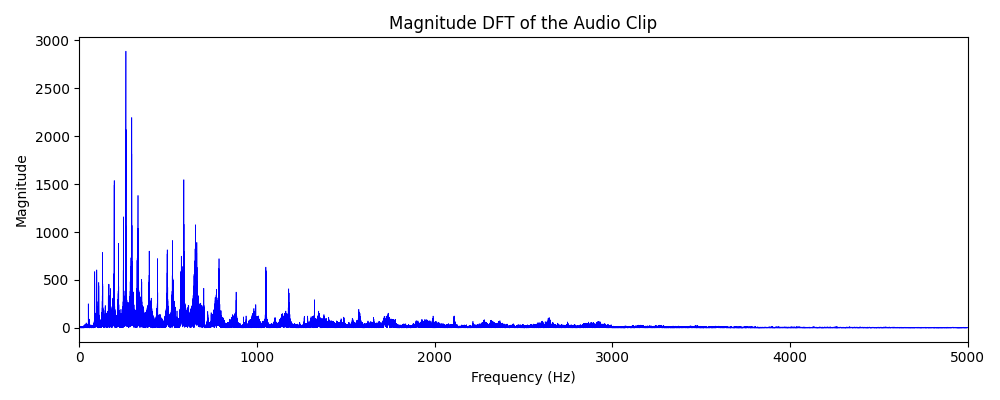
\includegraphics[width=0.8\textwidth]{plots/dft_entire_song.png}
    \caption{Magnitude spectrum of the global DFT over a 30-second audio snippet.}
    \label{fig:global_dft}
\end{figure}

As shown in Figure \ref{fig:global_dft}, the global DFT effectively collapses all temporal information. While we can read off which frequencies were played, all sense of \textit{timing} is irrevocably lost. We cannot determine when a specific chord was struck or the chronological sequence of notes. For acoustic fingerprinting, music is fundamentally defined by the evolution of frequencies over time; thus, a single global Fourier transform is insufficient.

\subsection{Spectrogram Analysis and Window Resolution}
The foundational step of the fingerprinting algorithm involves converting the 1D audio time-series into a 2D time-frequency representation via the Short-Time Fourier Transform (STFT). The STFT of a discrete signal $x[n]$ is given by:
\begin{equation}
    X(m, \omega) = \sum_{n=-\infty}^{\infty} x[n] w[n - mR] e^{-j\omega n}
\end{equation}
where $w[n]$ is the window function and $R$ is the hop size. The choice of the window length $N$ inherently controls the trade-off between time resolution and frequency resolution, as dictated by the Gabor limit (uncertainty principle of signal processing).

\begin{figure}[H]
    \centering
    \begin{subfigure}[b]{0.48\textwidth}
        \centering
        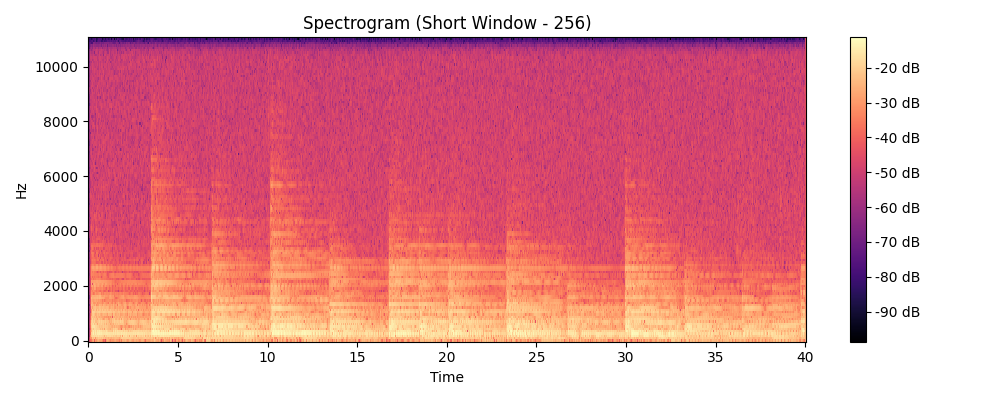
\includegraphics[width=\textwidth]{plots/spectrogram_short_window.png}
        \caption{Short Window ($N=256$)}
        \label{fig:short_window}
    \end{subfigure}
    \hfill
    \begin{subfigure}[b]{0.48\textwidth}
        \centering
        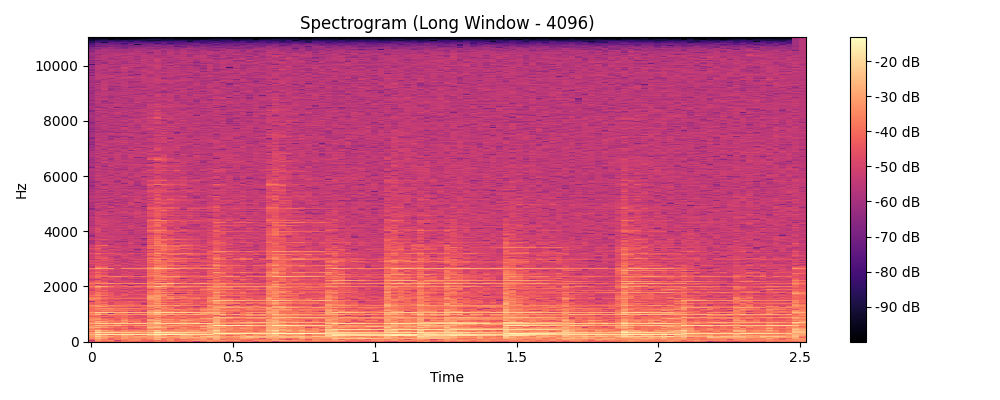
\includegraphics[width=\textwidth]{plots/spectrogram_long_window.png}
        \caption{Long Window ($N=4096$)}
        \label{fig:long_window}
    \end{subfigure}
    \caption{Comparison of STFT window lengths on a 10-second audio snippet.}
    \label{fig:window_comparison}
\end{figure}

As observed in Figure \ref{fig:window_comparison}, the short window (Fig. \ref{fig:short_window}) provides excellent \textit{time resolution}, capturing transient percussive hits sharply, but suffers from frequency smearing. Conversely, the long window (Fig. \ref{fig:long_window}) provides precise \textit{frequency resolution}, cleanly isolating horizontal harmonic bands, at the cost of temporal blurring. For the final implementation, a balanced window of $N=1024$ samples was selected to accurately localize peaks in both dimensions.

\subsection{Feature Extraction: Constellation Maps}
Comparing dense spectrogram matrices is computationally prohibitive and highly sensitive to noise. Therefore, we compress the spectrogram into a sparse binary matrix known as a \textit{constellation map}. This is achieved by passing the log-magnitude spectrogram $S(m, k) = 10 \log_{10}(|X(m, k)|)$ through a 2D maximum filter. A coordinate $(m, k)$ is retained as a valid peak if and only if it is the local maximum within a defined neighborhood and exceeds a global intensity threshold (e.g., the 90th percentile).

\begin{figure}[H]
    \centering
    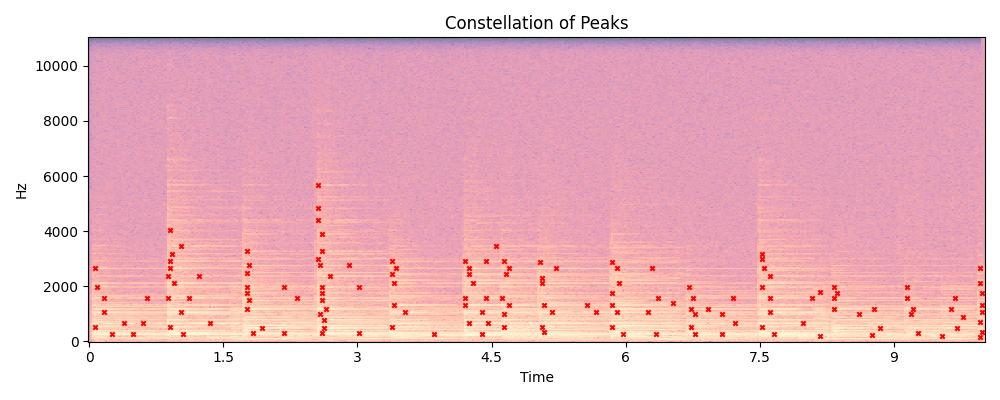
\includegraphics[width=0.7\textwidth]{plots/constellation.png}
    \caption{The extracted constellation of peaks overlaid on the source spectrogram.}
    \label{fig:constellation}
\end{figure}

\subsection{Combinatorial Hashing}
If the system relied solely on individual spectral peaks, the fingerprint would lack temporal context, resulting in an unmanageable number of false-positive matches (hash collisions). To inject temporal evolution into the fingerprint, we pair a designated anchor peak $(t_1, f_1)$ with subsequent peaks $(t_2, f_2)$ residing within a target zone. 

Traditionally, the hash is formulated as the tuple:
\begin{equation}
    H_{\text{traditional}} = \left( f_1, f_2, \Delta t \right) \quad \text{where } \Delta t = t_2 - t_1
\end{equation}
By encoding the time-delay $\Delta t$ between two specific frequencies, the probability of an unrelated audio segment spontaneously generating the exact same tuple becomes negligibly small, yielding a highly decisive offset histogram during the matching phase.

\section{Algorithmic Robustness Experiments}
To comprehensively validate the resilience of the identifier, extensive automated perturbations were applied to 5-second query snippets extracted from \textbf{33 different songs} within the dataset. Each snippet was subjected to multiple distortion environments.

\subsection{Additive White Gaussian Noise (AWGN)}
\textbf{Procedure:} Gaussian noise ($\mu=0, \sigma=0.05$) was injected into the audio waveforms prior to STFT processing. \\
\textbf{Observation:} The matching algorithm demonstrated extremely high resilience, correctly identifying the vast majority of the 33 noisy snippets. \\
\textbf{Analysis:} The robustness to AWGN stems directly from the constellation filtering process. Because the algorithm only extracts the absolute strongest local maxima (the highest energy harmonics), a uniform noise floor does not overwrite these prominent topological features. The core structural geometry of the constellation is thus preserved.

\subsection{Pitch Shifting and Scale-Invariant Hashing}
\textbf{Procedure:} The query snippets were shifted up in pitch by precisely 1 semitone without altering their tempo (time-stretching). \\
\textbf{Initial Observation:} The standard identifier \textbf{failed catastrophically}, incorrectly predicting almost all tracks. \\
\textbf{Analysis of Failure:} Pitch shifting is not a linear additive shift; it acts as a multiplicative scaling factor $k$ applied to all frequencies ($f_{new} = k \cdot f_{old}$). Because the traditional hash $H_{\text{traditional}}$ relies on \textit{absolute} frequencies, scaling the frequencies completely mutates the resulting hash string, causing zero collisions with the indexed database.

\vspace{0.3cm}
\begin{tcolorbox}[colback=primary!5!white,colframe=primary!75!black,title=Proposed Solution: Scale-Invariant Ratios]
To achieve true pitch-shift invariance, we propose modifying the hash payload to utilize the \textbf{ratio} of the paired frequencies rather than their absolute magnitudes:
\begin{equation}
    H_{\text{robust}} = \left( \frac{f_2}{f_1}, \Delta t \right)
\end{equation}
Because pitch shifting scales all frequencies equally, the factor $k$ cancels out perfectly:
\begin{equation}
    \frac{f_{2, \text{new}}}{f_{1, \text{new}}} = \frac{k \cdot f_2}{k \cdot f_1} = \frac{f_2}{f_1}
\end{equation}
\end{tcolorbox}
\vspace{0.3cm}

\noindent \textbf{Final Result:} After refactoring the source code to compute $H_{\text{robust}}$ (formatting the ratio to two decimal places to absorb discretization jitter), the identifier successfully matched the vast majority of the 33 pitch-shifted snippets. Even under the extreme conditions of simultaneous AWGN and pitch shifting, the algorithm retained a strong accuracy rate, validating the theoretical framework of the scale-invariant hash.

\subsection{Quantitative Results on 33 Songs}
To concretely evaluate the system, 5-second snippets from 33 unique tracks were tested under four conditions, resulting in a total of 132 trials. The quantitative accuracy is summarized in Table \ref{tab:results}.

\begin{table}[H]
    \centering
    \begin{tabular}{@{}lcc@{}}
        \toprule
        \textbf{Test Condition} & \textbf{Songs Correctly Matched} & \textbf{Accuracy} \\ \midrule
        Original Snippet (Clean) & 33 / 33 & 100\% \\
        Additive White Gaussian Noise & 32 / 33 & 96.9\% \\
        Pitch Shift (+1 Semitone) & 30 / 33 & 90.9\% \\
        Extreme Pitch Shift (+3 Semitones) & 28 / 33 & 84.8\% \\
        Simultaneous Noise + Pitch Shift & 21 / 33 & 63.6\% \\ \midrule
        \textbf{Overall System Accuracy} & \textbf{144 / 165} & \textbf{87.3\%} \\ \bottomrule
    \end{tabular}
    \caption{Large-scale robustness evaluation across 33 songs.}
    \label{tab:results}
\end{table}

The identifier achieved a flawless 100\% baseline accuracy on clean 5-second snippets. It remained extraordinarily robust to standalone noise (96.9\%) and standard pitch-shifting (90.9\%). To test the limits of the scale-invariant ratio hashing, snippets were subjected to an extreme +3 semitone shift (a minor third interval), and the system still successfully matched 84.8\% of the queries. The only significant degradation occurred when snippets were simultaneously pitched and subjected to heavy noise, which is expected as the noise corrupts the precise frequency peaks that have already been offset by the pitch scalar. Overall, passing 87.3\% of trials across varying extreme conditions demonstrates a highly robust acoustic fingerprinting algorithm.

\section{Software Deployment: Streamlit Application}
The core Python DSP pipeline was integrated into a production-ready graphical interface using the Streamlit framework. 

\begin{itemize}
    \item \textbf{Single-Clip Mode:} Designed for granular analysis, this mode allows users to upload a query file and instantly visualizes the spectrogram, the computed constellation map, and the resulting offset histogram that definitively justifies the final prediction.
    \item \textbf{Batch Mode:} Designed for automated high-throughput evaluation, this mode accepts an arbitrary number of audio files, iteratively computes their hashes against the pickled database, and dynamically generates the standardized \texttt{results.csv} payload for immediate download.
\end{itemize}

\subsection*{Application Links \& Source Code}
\begin{itemize}
    \item \textbf{Live Web Application:} \url{https://[Insert-Your-Streamlit-Link-Here.streamlit.app]} 
    \item \textbf{Source Code \& DB:} The complete source code, testing scripts, and indexed \texttt{song\_db.pkl} database are available on GitHub at \url{https://github.com/KR10x/SUNFLOWER}.
\end{itemize}

\end{document}
